% Relatório da Entrega 1 — Projeto e Arquitetura de Software (PUCRS)
% Baseado no Modelo Canônico de Trabalhos Acadêmicos com abnTeX2
\documentclass[
	12pt,
	oneside,
	a4paper,
	chapter=TITLE,
	section=TITLE,
	sumario=tradicional,
	english,
	brazil
]{abntex2}

\usepackage{lmodern}
\usepackage[T1]{fontenc}
\usepackage[utf8]{inputenc}
\usepackage{indentfirst}
\usepackage{color}
\usepackage{graphicx}
\usepackage{microtype}
\usepackage{xcolor}
\usepackage{listings}
\usepackage{booktabs}
\usepackage{float}
\usepackage{tikz}
\usetikzlibrary{arrows.meta,positioning,shapes.geometric,fit,backgrounds}

\usepackage[brazilian,hyperpageref]{backref}
\usepackage[alf]{abntex2cite}

\renewcommand{\backrefpagesname}{Citado na(s) página(s):~}
\renewcommand{\backref}{}
\renewcommand*{\backrefalt}[4]{
	\ifcase #1
		Nenhuma citação no texto.
	\or
		Citado na página #2.
	\else
		Citado #1 vezes nas páginas #2.
	\fi}

\definecolor{bgcode}{RGB}{245,245,245}
\lstset{
  basicstyle=\ttfamily\footnotesize,
  backgroundcolor=\color{bgcode},
  frame=single,
  breaklines=true,
  columns=fullflexible,
  showstringspaces=false
}

% ---------------------------------------------------------------------------
% Informações de dados para CAPA e FOLHA DE ROSTO
% ---------------------------------------------------------------------------
\titulo{Integração i-Educar $\rightarrow$ Moodle}
\autor{Airton Luiz Canale Filho \\ João Pedro Ayache}
% Para incluir mais autores, use: \autor{Nome Um \\ Nome Dois}
\local{Porto Alegre}
\data{2026}
\orientador[Professor:]{José Pedro Schardosim Simão}
\instituicao{%
  Pontifícia Universidade Católica do Rio Grande do Sul -- PUCRS
  \par
  Escola Politécnica
  \par
  Projeto e Arquitetura de Software}
\tipotrabalho{Relatório técnico}
\preambulo{Relatório da Entrega 1 da disciplina Projeto e Arquitetura de Software,
apresentando a implementação de uma integração monolítica entre o i-Educar e o Moodle.}

\definecolor{blue}{RGB}{41,5,195}
\makeatletter
\hypersetup{
	pdftitle={\@title},
	pdfauthor={\@author},
	pdfsubject={\imprimirpreambulo},
	pdfcreator={LaTeX with abnTeX2},
	pdfkeywords={i-Educar}{Moodle}{integração}{arquitetura de software},
	colorlinks=true,
	linkcolor=blue,
	citecolor=blue,
	filecolor=magenta,
	urlcolor=blue,
	bookmarksdepth=4
}
\makeatother

\setlength{\parindent}{1.3cm}
\setlength{\parskip}{0.2cm}

\makeindex

\begin{document}

\selectlanguage{brazil}
\frenchspacing

% ---------------------------------------------------------------------------
% ELEMENTOS PRÉ-TEXTUAIS
% ---------------------------------------------------------------------------
\imprimircapa
\imprimirfolhaderosto*

\setlength{\absparsep}{18pt}
\begin{resumo}
Este relatório descreve a arquitetura e a implementação de uma integração monolítica entre o
\emph{i-Educar} e o \emph{Moodle}, feita como aplicação Python modular. A solução
sincroniza turmas e vínculos (matrículas e professorados) de forma síncrona e idempotente,
usando o campo \texttt{idnumber} do Moodle como chave de correlação. Todo o ambiente é
orquestrado em um único \texttt{docker-compose} que inclui o i-Educar, o Moodle e a
aplicação de integração.

\textbf{Palavras-chave}: i-Educar. Moodle. Integração de sistemas. Monólito modular.
\end{resumo}

\pdfbookmark[0]{\listfigurename}{lof}
\listoffigures*
\cleardoublepage

\pdfbookmark[0]{\listtablename}{lot}
\listoftables*
\cleardoublepage

\pdfbookmark[0]{\contentsname}{toc}
\tableofcontents*
\cleardoublepage

% ---------------------------------------------------------------------------
% ELEMENTOS TEXTUAIS
% ---------------------------------------------------------------------------
\textual

\chapter{Objetivo}

Integrar o sistema de gestão escolar \emph{i-Educar}~\cite{ieducar} ao ambiente de
aprendizagem \emph{Moodle}~\cite{moodle-ws}, de modo que turmas cadastradas no i-Educar passem a existir como cursos no
Moodle, com os alunos matriculados e os professores vinculados. A operação deve ser
executada sob demanda via API HTTP e também periodicamente por agendador interno,
preservando idempotência (nova execução não duplica dados).

\chapter{Informações sincronizadas}

\begin{itemize}
    \item \textbf{Turmas} do i-Educar $\rightarrow$ \textbf{Cursos} no Moodle (campo
    \texttt{idnumber = ieducar-turma-\{id\}}).
    \item \textbf{Pessoas vinculadas} (alunos matriculados e professores) $\rightarrow$
    \textbf{Usuários} no Moodle, criados sob demanda (\texttt{idnumber =
    ieducar-pessoa-\{id\}}).
    \item \textbf{Vínculos} (matrícula ativa, professorado) $\rightarrow$ \textbf{Inscrições}
    no curso Moodle correspondente, com papel \texttt{student} ou \texttt{editingteacher}.
    \item Metadados de execução ficam no Postgres da integração em três tabelas:
    \texttt{MapeamentoExterno} (dedup), \texttt{ExecucaoSync} (auditoria) e
    \texttt{FalhaSync} (erros individuais).
\end{itemize}

\chapter{Arquitetura}

A solução segue o estilo \emph{monólito modular}: um único deployable Python
(FastAPI~\cite{fastapi} e SQLAlchemy~\cite{sqlalchemy}) organizado
em domínios bem delimitados, com portas e adaptadores entre o núcleo de negócio e as
infraestruturas externas (i-Educar e Moodle). A Figura~\ref{fig:componentes} mostra os
componentes principais.

\begin{figure}[H]
\centering
\resizebox{\textwidth}{!}{%
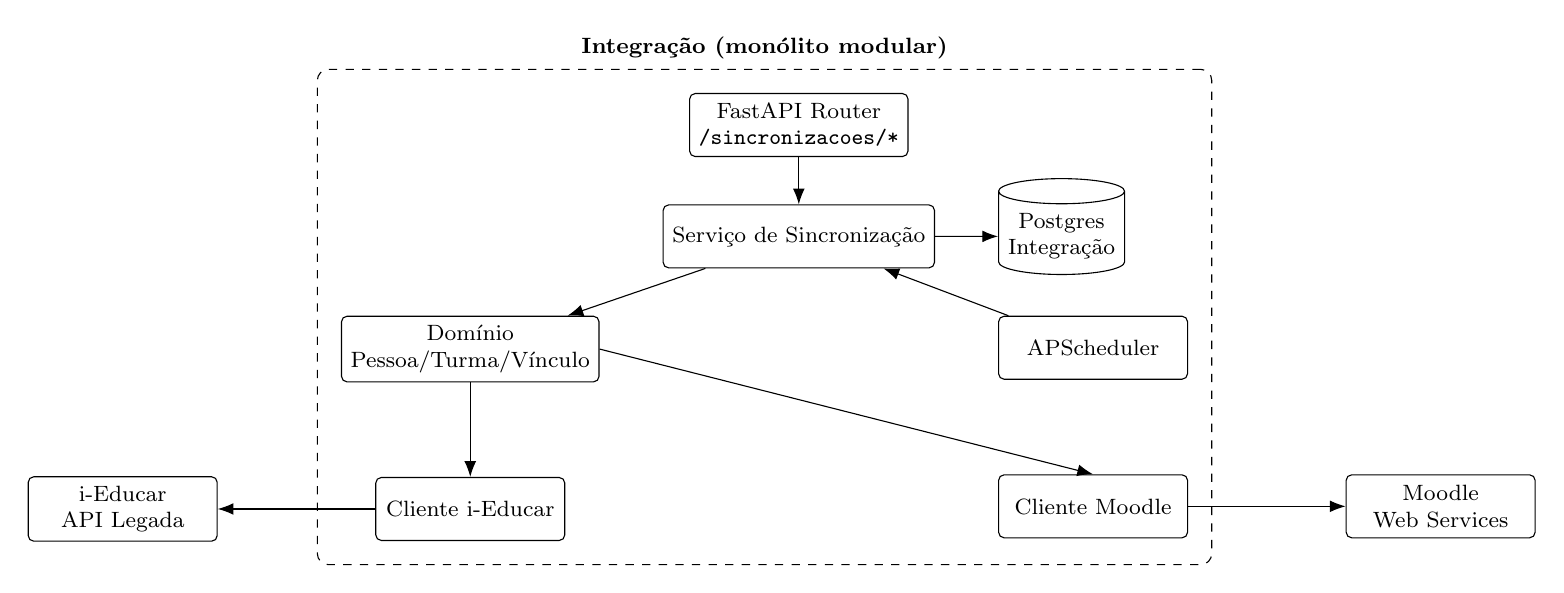
\begin{tikzpicture}[
    node distance=0.6cm and 0.8cm,
    box/.style={rectangle, draw, rounded corners=2pt, minimum height=0.8cm, minimum width=2.4cm, align=center, font=\footnotesize},
    db/.style={cylinder, draw, shape border rotate=90, aspect=0.2, minimum height=1cm, minimum width=1.6cm, align=center, font=\footnotesize},
    group/.style={draw, dashed, inner sep=0.3cm, rounded corners},
    arr/.style={-{Latex[length=2mm]}}
]
    \node[box] (api) {FastAPI Router\\\texttt{/sincronizacoes/*}};
    \node[box, below=of api] (svc) {Serviço de Sincronização};
    \node[box, below left=of svc] (dompes) {Domínio\\Pessoa/Turma/Vínculo};
    \node[box, below right=of svc] (sched) {APScheduler};
    \node[box, below=1.2cm of dompes] (cliie) {Cliente i-Educar};
    \node[box, below=1.2cm of sched] (climd) {Cliente Moodle};
    \node[db, right=of svc] (repo) {Postgres\\Integração};

    \node[box, left=2cm of cliie] (ie) {i-Educar\\API Legada};
    \node[box, right=2cm of climd] (md) {Moodle\\Web Services};

    \begin{scope}[on background layer]
        \node[group, fit=(api)(svc)(dompes)(sched)(cliie)(climd)(repo), label=above:{\footnotesize\textbf{Integração (monólito modular)}}] {};
    \end{scope}

    \draw[arr] (api) -- (svc);
    \draw[arr] (sched) -- (svc);
    \draw[arr] (svc) -- (dompes);
    \draw[arr] (svc) -- (repo);
    \draw[arr] (dompes) -- (cliie);
    \draw[arr] (dompes.east) -- (climd.north);
    \draw[arr] (cliie) -- (ie);
    \draw[arr] (climd) -- (md);
\end{tikzpicture}%
}
\caption{Componentes principais e dependências externas.}
\label{fig:componentes}
\end{figure}

\section{Separação de responsabilidades}

\begin{description}
    \item[\texttt{app/dominios/}] Regras de negócio puras (modelos, serviços, portas).
    Não importa HTTP nem SQL. Define \emph{o que} precisa acontecer.
    \item[\texttt{app/infraestrutura/}] Adaptadores concretos: cliente HTTP para i-Educar
    (com tradutor de payloads para múltiplas versões), cliente REST para Moodle, e
    implementações \emph{fake} em memória usadas em dev e testes.
    \item[\texttt{app/dominios/sincronizacao/}] Orquestração: carrega dados do i-Educar,
    confere mapeamento no banco, chama Moodle quando necessário, registra execução e
    falhas.
    \item[\texttt{app/composicao.py}] \emph{Composition root} --- escolhe entre cliente
    real e \emph{fake} conforme \texttt{.env}.
    \item[\texttt{app/main.py}] \emph{Entrypoint} FastAPI, cria \emph{schema} no boot e
    inicia o agendador.
\end{description}

\section{Interfaces}

As portas de domínio são \texttt{Protocol}s Python (duck-typing estrutural). A
Tabela~\ref{tab:portas} resume as principais.

\begin{table}[H]
\centering
\footnotesize
\begin{tabular}{lll}
\toprule
Porta & Métodos & Implementações \\
\midrule
\texttt{ClienteIEducar} & \texttt{listar\_turmas, listar\_vinculos, obter\_pessoa} & \texttt{http}, \texttt{fake} \\
\texttt{ClienteMoodle}  & \texttt{criar\_curso, upsert\_usuario, inscrever}         & \texttt{http}, \texttt{fake} \\
\texttt{ExecucaoRepo}   & \texttt{criar, finalizar, registrar\_falha, listar, obter} & SQLAlchemy \\
\texttt{MapeamentoRepo} & \texttt{buscar, registrar}                                & SQLAlchemy \\
\bottomrule
\end{tabular}
\caption{Portas e implementações.}
\label{tab:portas}
\end{table}

\chapter{Diagrama de fluxo}

\begin{figure}[H]
\centering
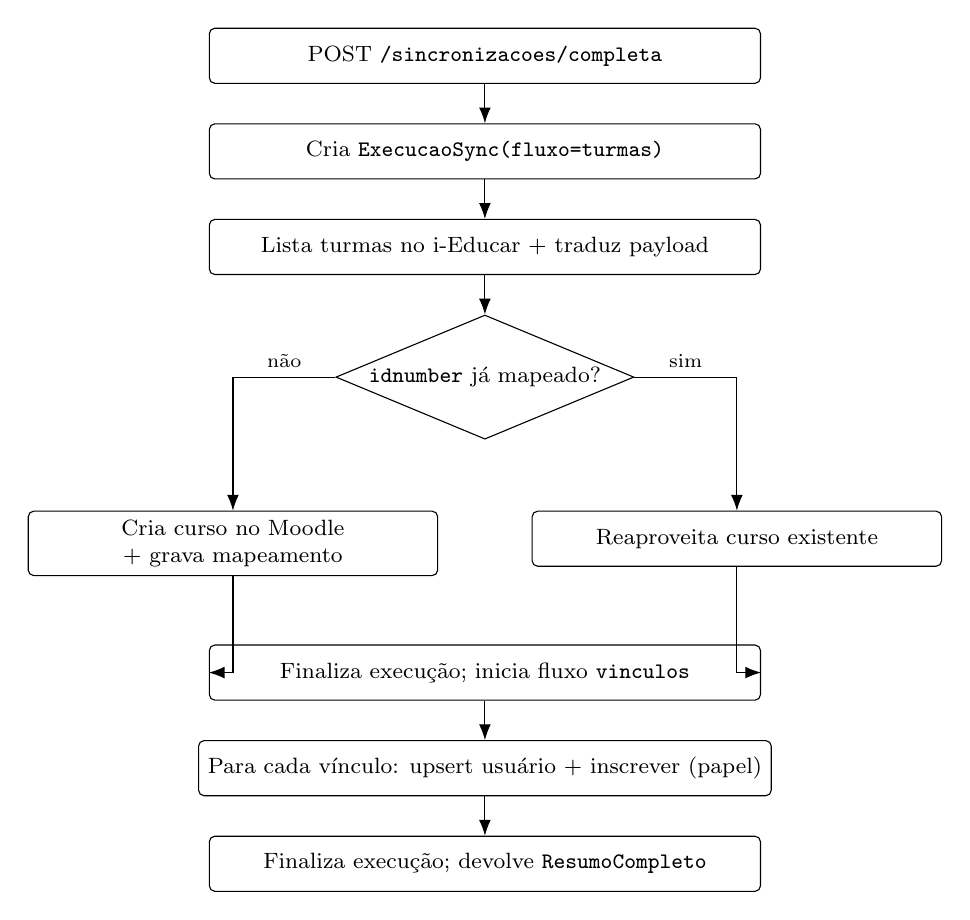
\begin{tikzpicture}[
    node distance=0.5cm,
    passo/.style={rectangle, draw, rounded corners=2pt, minimum height=0.7cm, minimum width=7cm, align=center, font=\footnotesize},
    dec/.style={diamond, draw, aspect=2.4, minimum height=0.7cm, align=center, font=\footnotesize, inner sep=1pt},
    arr/.style={-{Latex[length=2mm]}}
]
    \node[passo] (s1) {POST \texttt{/sincronizacoes/completa}};
    \node[passo, below=of s1] (s2) {Cria \texttt{ExecucaoSync(fluxo=turmas)}};
    \node[passo, below=of s2] (s3) {Lista turmas no i-Educar + traduz payload};
    \node[dec, below=of s3] (d1) {\texttt{idnumber} já mapeado?};
    \node[passo, minimum width=5.2cm, below=0.9cm of d1, xshift=-3.2cm] (s4) {Cria curso no Moodle\\+ grava mapeamento};
    \node[passo, minimum width=5.2cm, below=0.9cm of d1, xshift=3.2cm] (s5) {Reaproveita curso existente};
    \node[passo, below=2.6cm of d1] (s6) {Finaliza execução; inicia fluxo \texttt{vinculos}};
    \node[passo, below=of s6] (s7) {Para cada vínculo: upsert usuário + inscrever (papel)};
    \node[passo, below=of s7] (s8) {Finaliza execução; devolve \texttt{ResumoCompleto}};

    \draw[arr] (s1) -- (s2);
    \draw[arr] (s2) -- (s3);
    \draw[arr] (s3) -- (d1);
    \draw[arr] (d1.west) -| node[above,pos=0.25,font=\scriptsize]{não} (s4.north);
    \draw[arr] (d1.east) -| node[above,pos=0.25,font=\scriptsize]{sim} (s5.north);
    \draw[arr] (s4.south) |- (s6.west);
    \draw[arr] (s5.south) |- (s6.east);
    \draw[arr] (s6) -- (s7);
    \draw[arr] (s7) -- (s8);
\end{tikzpicture}
\caption{Fluxo de sincronização completa (turmas + vínculos).}
\label{fig:fluxo}
\end{figure}

\chapter{Decisões técnicas}

\begin{description}
    \item[Monólito modular (não microserviços).] Escopo pequeno, deploy único, latência
    menor; a modularidade por portas mantém o custo de evolução baixo.
    \item[Sincronização síncrona com Postgres de controle.] O enunciado exige fluxo
    síncrono. Três tabelas (\texttt{ExecucaoSync}, \texttt{FalhaSync},
    \texttt{MapeamentoExterno}) bastam para auditoria e idempotência, sem introduzir fila.
    \item[\texttt{idnumber} prefixado como chave de correlação.] Campo nativo do Moodle,
    não exige alterar schema do i-Educar. Prefixos (\texttt{ieducar-turma-},
    \texttt{ieducar-pessoa-}) tornam a origem explícita.
    \item[Clientes \emph{http} e \emph{fake} atrás da mesma porta.] O \emph{fake} com
    dados seed habilita desenvolvimento sem subir i-Educar/Moodle e sustenta testes E2E
    determinísticos.
    \item[\texttt{httpx} com \emph{retry}/\emph{backoff} e classificação de erro.] Erros
    transitórios dos dois sistemas são comuns; a camada HTTP separa falha fatal de
    retriável sem contaminar o domínio.
    \item[APScheduler \emph{in-process}.] Sem dependências externas (Redis, Celery). A
    limitação (uma instância só) é aceita conscientemente para o escopo da entrega.
    \item[Tradutor dedicado para payloads do i-Educar.] A API legada varia nomes de campos
    entre versões; o tradutor isola essa normalização num ponto só.
    \item[\texttt{docker-compose} unificado via \texttt{include:}.] Um único
    \texttt{docker compose up} sobe i-Educar, Moodle e a integração. O Moodle está
    versionado em \texttt{infra/moodle/}; o i-Educar oficial é obtido por
    \texttt{make infra} em uma versão fixada, sem copiar seu código para o repositório.
\end{description}

\chapter{Testes realizados}

\begin{itemize}
    \item \textbf{Unitários de domínio} (\texttt{tests/test\_pessoa.py}): regras de nome,
    \emph{username}, email sintético e \texttt{idnumber}.
    \item \textbf{Tradutor} (\texttt{tests/test\_tradutor.py}): cobre variantes de campos
    de turmas e vínculos entre versões do i-Educar.
    \item \textbf{Orquestração E2E com \emph{fakes}} (\texttt{tests/test\_sincronizacao.py}):
    idempotência (segunda rodada não cria nada), inativação (remove inscrição),
    atribuição de papéis, e caminhos de falha gravando em \texttt{FalhaSync}.
    \item \textbf{Endpoints HTTP} (\texttt{tests/test\_api.py}): via FastAPI
    \texttt{TestClient} com \emph{dependency overrides} e \texttt{lru\_cache} invalidado.
\end{itemize}

Comando: \texttt{pytest}. A suíte tem 24 testes, todos passando, e roda sem exigir rede
ou containers externos.

\chapter{Resultados}

A integração sincroniza turmas e vínculos de uma escola/ano a cada requisição a
\texttt{POST /sincronizacoes/completa}, devolvendo um resumo com contagens de
\texttt{processados}, \texttt{criados}, \texttt{reaproveitados} e \texttt{falhas}. Rodando
duas vezes seguidas sobre a mesma base, a segunda execução reporta \texttt{criados = 0} e
tudo em \texttt{reaproveitados}, confirmando idempotência via \texttt{MapeamentoExterno} e
\texttt{idnumber}. O agendador interno repete o fluxo completo a cada
\texttt{AGENDADOR\_INTERVALO\_MIN} minutos. Falhas individuais em pessoas/turmas não
abortam a execução: ficam registradas em \texttt{FalhaSync} e o resumo marca o
\texttt{status} apropriado.

\section{Evidências de execução}

As evidências a seguir foram obtidas executando a aplicação real (FastAPI, serviço de
sincronização e banco de controle) com os adaptadores \emph{fake} do i-Educar e do Moodle
(\texttt{IEDUCAR\_CLIENTE=fake}, \texttt{MOODLE\_CLIENTE=fake}), que simulam em memória
duas turmas e quatro vínculos. As respostas da API foram salvas em
\texttt{docs/evidencias/}. A Tabela~\ref{tab:evidencias} resume as duas execuções
consecutivas de \texttt{POST /sincronizacoes/completa?ano=2025}.

\begin{table}[H]
\centering
\footnotesize
\begin{tabular}{llrrrr}
\toprule
Rodada & Fluxo & Processados & Criados & Reaproveitados & Falhas \\
\midrule
1ª & turmas   & 2 & 2 & 0 & 0 \\
1ª & vínculos & 4 & 4 & 0 & 0 \\
2ª & turmas   & 2 & 0 & 2 & 0 \\
2ª & vínculos & 4 & 0 & 4 & 0 \\
\bottomrule
\end{tabular}
\caption{Resumo das duas execuções consecutivas da sincronização completa.}
\label{tab:evidencias}
\end{table}

A segunda rodada não cria nenhum registro novo e reaproveita todos os existentes,
evidenciando a idempotência. A Figura~\ref{fig:painel} mostra o painel web da integração
com o histórico dessas quatro execuções.

\begin{figure}[H]
\centering
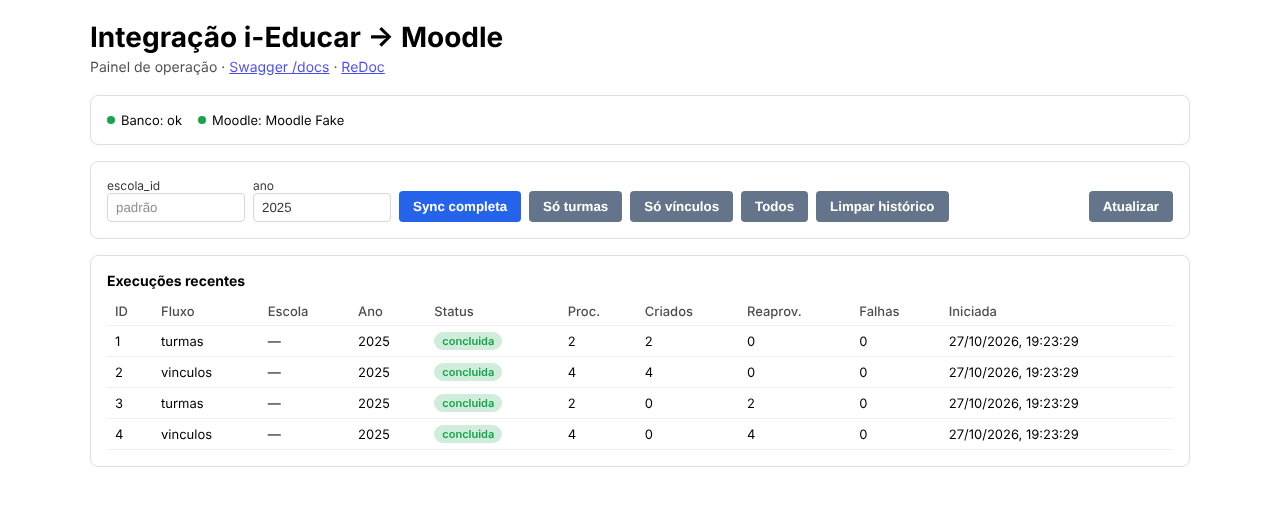
\includegraphics[width=\textwidth]{painel.png}
\caption{Painel da integração com o histórico das execuções.}
\label{fig:painel}
\end{figure}

\chapter{Limitações}

\begin{itemize}
    \item \texttt{FalhaSync} é persistida mas não há endpoint de reprocessamento
    automático --- requer re-executar o fluxo completo.
    \item O \emph{schema} é criado via \texttt{Base.metadata.create\_all} no \emph{boot};
    não há Alembic nem versionamento de migrações.
    \item A API da integração não exige autenticação --- assume execução em rede interna
    confiável (do \emph{compose}).
    \item O agendador é \emph{single-instance}; duas instâncias simultâneas rodariam o
    mesmo \emph{job} em paralelo (sem \emph{lock} distribuído).
    \item A exclusão lógica de turmas no i-Educar remove inscrições mas não arquiva o
    curso no Moodle.
\end{itemize}

\chapter{Repositório e execução}

Instruções completas de \emph{setup}, geração de credenciais (\texttt{IEDUCAR\_ACCESS\_KEY}
e \texttt{MOODLE\_TOKEN}) e demonstração estão no \texttt{README.md} do repositório. O
caminho rápido é:

\begin{lstlisting}[language=bash]
make infra
cp .env.example .env
docker compose up -d --build
make ieducar-install
# gerar tokens, colar em .env, docker compose restart integracao
curl -X POST "http://localhost:8000/sincronizacoes/completa?escola_id=1&ano=2025"
\end{lstlisting}

% ---------------------------------------------------------------------------
% ELEMENTOS PÓS-TEXTUAIS
% ---------------------------------------------------------------------------
\postextual

\bibliography{referencias}

\end{document}
